\chapter{Movimentos de Fim de Jogo}

A posição no \emph{Dia.\@~1} abaixo é a mesma que no \emph{Dia.\@~6} do \autoref{chap:estrat_comp} após Branco ter jogado 13 (a pedra marcada). Quando Preto desce para 1 (14 no \emph{Dia.\@~6} do \autoref{chap:estrat_comp}), Branco não deveria jogar em outro lugar, com 2 por exemplo, já que Preto invadirá com 3, e Branco não conseguirá defender seu território.

\begin{figure}[h!]
    \centering
    \begin{subfigure}[t]{.475\textwidth}
        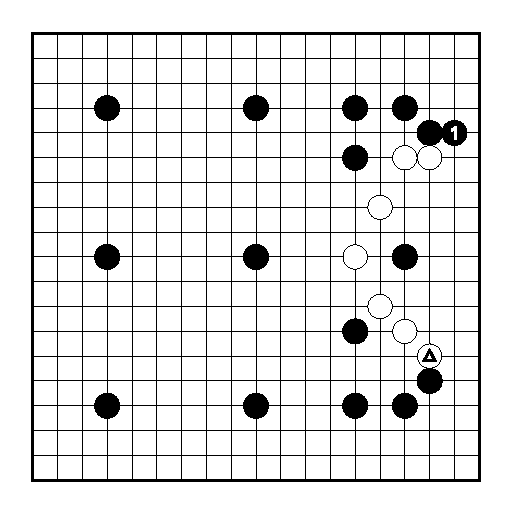
\includegraphics[width=1\textwidth]{11 - Dia 1}
        \captionsetup{justification=centering}
        \caption*{\emph{Dia.\@~1}}
    \end{subfigure}
    \hfill
    \begin{subfigure}[t]{.475\textwidth}
        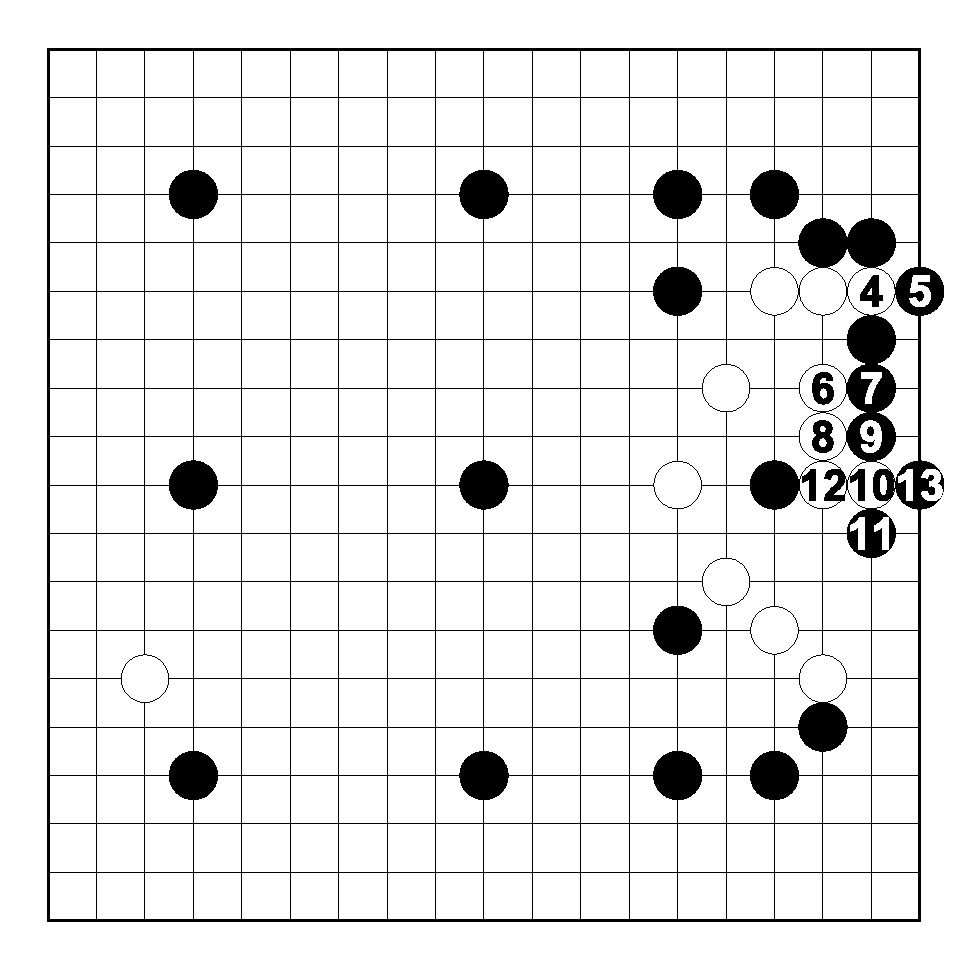
\includegraphics[width=1\textwidth]{11 - Dia 2}
        \captionsetup{justification=centering}
        \caption*{\emph{Dia.\@~2}}
    \end{subfigure}
\end{figure}

O melhor que ele pode fazer, no caso da invasão, é empurrar com 4 no \emph{Dia.\@~2} e pular para 6. Porém, Preto pode reduzir Branco rastejando com 7 a 9. Após os movimentos até 13, o território branco basicamente desapareceu. Branco investiu movimentos demais nesta área para deixar que isso ocorra.

\pagebreak

\begin{wrapfigure}{r}{60mm}
    \vspace{-20pt}
    \begin{center}
        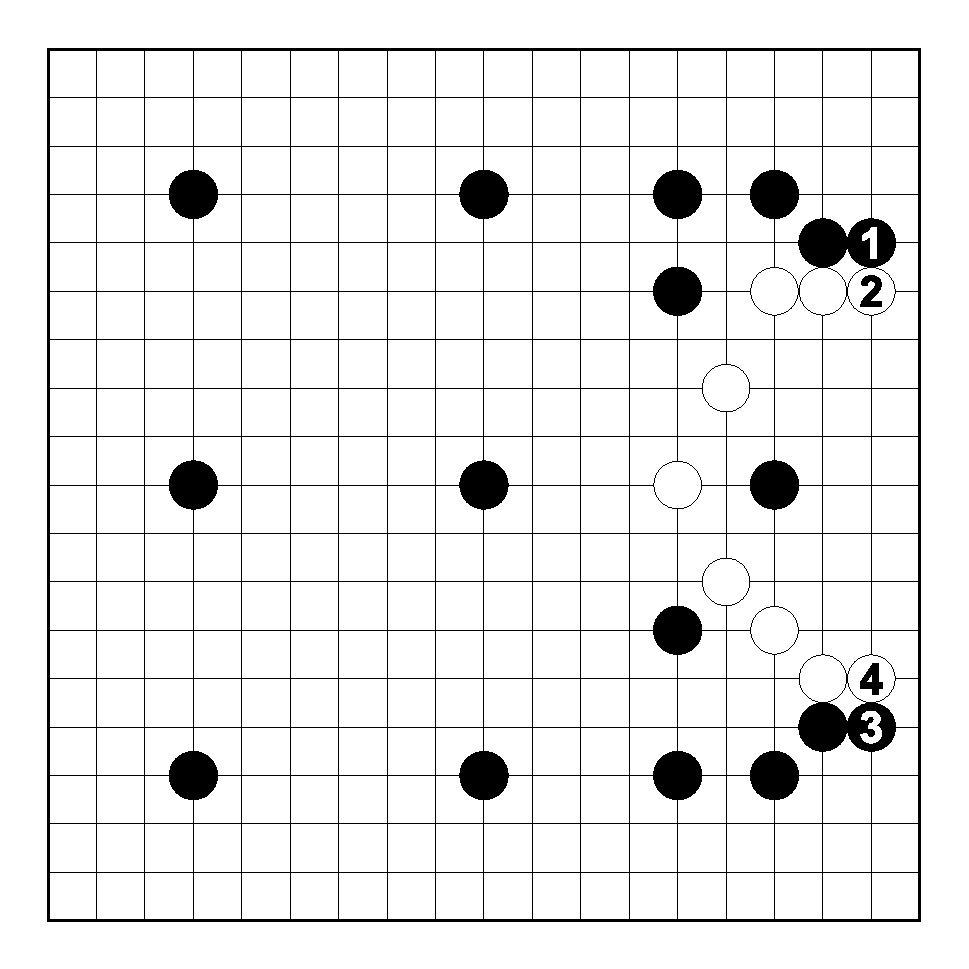
\includegraphics[width=.5\textwidth]{11 - Dia 3}
        \captionsetup{justification=centering}
        \caption*{\emph{Dia.\@~3}}
    \end{center}
    \vspace{-31pt}
\end{wrapfigure}

Sendo assim, quando Preto desce para 1 no \emph{Dia.\@~3}, Branco não possui nenhuma outra escolha senão defender com 2. Quando Preto desce para 3, ele precisa bloquear com 4 também.

Movimentos como Preto 1 e 3 são geralmente jogados no final do meio de jogo quando o território de cada lado já foi essencialmente determinado. Eles são utilizados para expandir territórios ao mesmo tempo que diminuem os do adversário. Em seguida\ldots

\pagebreak

Preto joga 5 e 7 no \emph{Dia.\@~4}, forçando Preto a defender com 6 e 8. Ele continua com o mesmo tipo de movimento na parte inferior do lado direito com 9 e 11, e Branco precisa defender com 12, terminando em \emph{gote}. Em outras palavras, Branco precisa fazer o último movimento defensivo.

\begin{figure}[h!]
    \centering
    \begin{subfigure}[t]{.475\textwidth}
        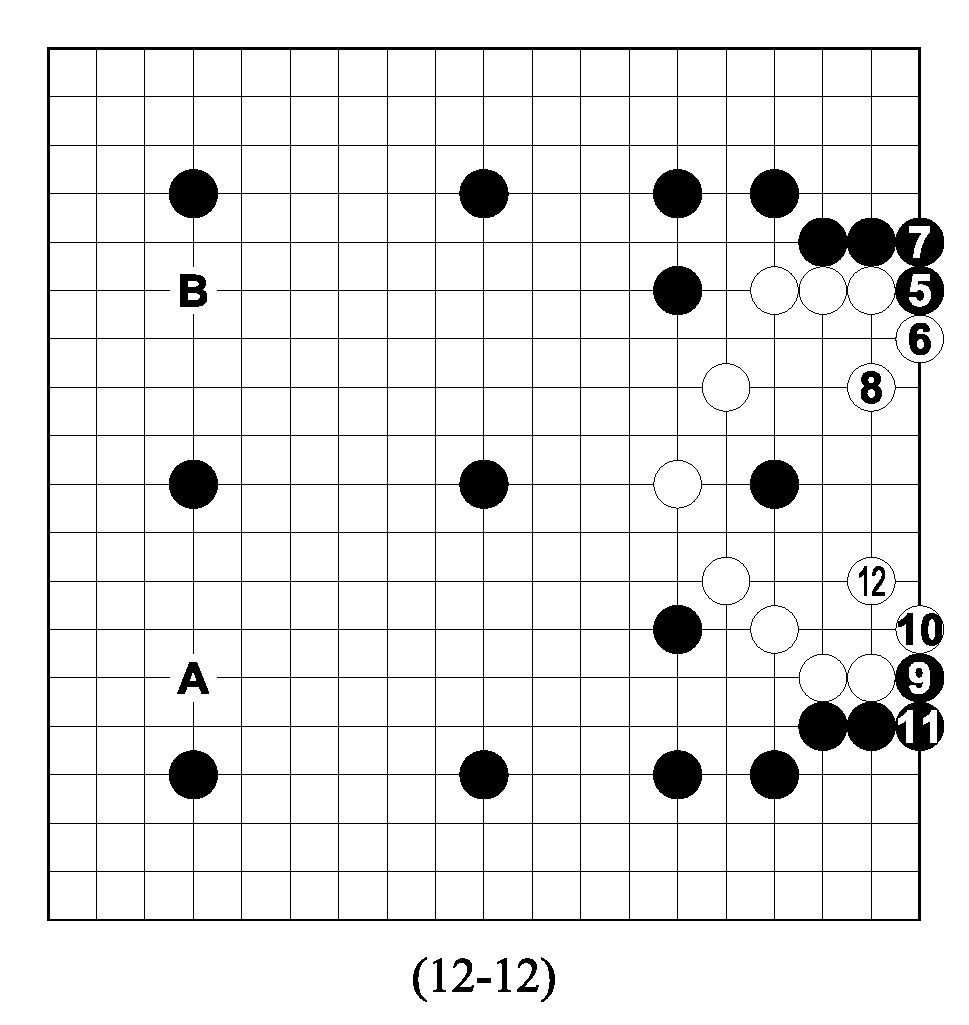
\includegraphics[width=1\textwidth]{11 - Dia 4}
        \captionsetup{justification=centering}
        \caption*{\emph{Dia.\@~4}}
    \end{subfigure}
    \hfill
    \begin{subfigure}[t]{.475\textwidth}
        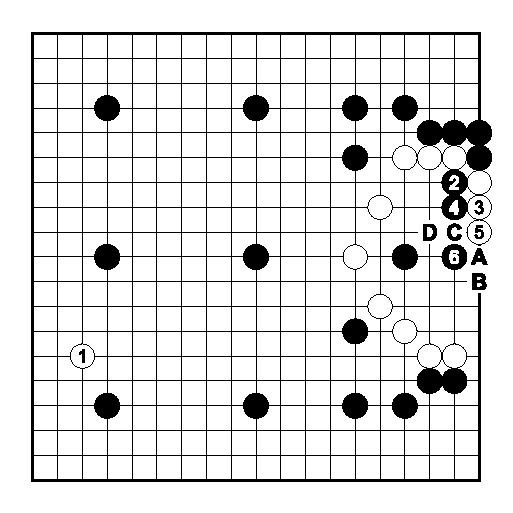
\includegraphics[width=1\textwidth]{11 - Dia 5}
        \captionsetup{justification=centering}
        \caption*{\emph{Dia.\@~5}}
    \end{subfigure}
\end{figure}

Por que Branco 8 e 12 seriam necessários?

Depois de Branco 12 no \emph{Dia.\@~4}, Preto possui sente. Isto é, ele possui a iniciativa --- ele não precisa defender e pode jogar onde quiser. Nesta posição, ele talvez queira jogar em \textbf{A} ou \textbf{B} e conseguiu uma boa vantagem nesta parte do tabuleiro.

Se Branco omitir 8 no \emph{Dia.\@~4} e se aproximar da pedra preta no canto inferior esquerdo com 1 no \emph{Dia.\@~5}, Preto cortará com 2. Se Branco tentar escapar com 3, Preto faz atari de novo com 4 e, então, enreda com 6. As pedras brancas não conseguem fugir. Se Branco \textbf{A}, Preto faz atari em \textbf{B}; se Branco \textbf{C}, Preto \textbf{D}.

\pagebreak

\section{Cálculos de Fim de Jogo}

Restrinjamos nossa atenção ao lado direito do tabuleiro, assumindo que os outros territórios no tabuleiro já foram decididos. Qual é o valor dos movimentos Preto 5 e 7? E qual é o valor dos movimentos Preto 9 e 11?

\begin{figure}[h!]
    \centering
    \begin{subfigure}[t]{.3\textwidth}
        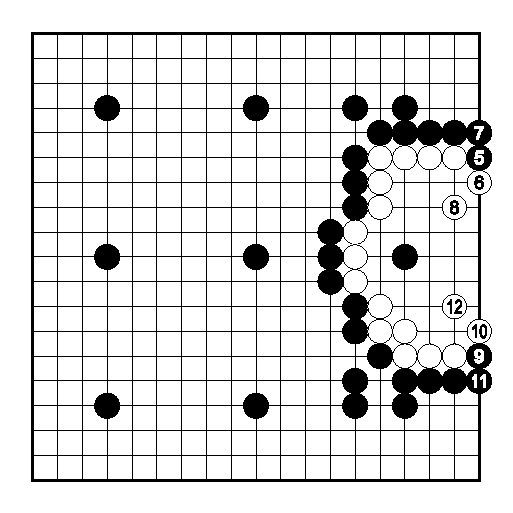
\includegraphics[width=1\textwidth]{11 - Dia 6}
        \captionsetup{justification=centering}
        \caption*{\emph{Dia.\@~6}}
    \end{subfigure}
    \hspace{1cm}
    \begin{subfigure}[t]{.3\textwidth}
        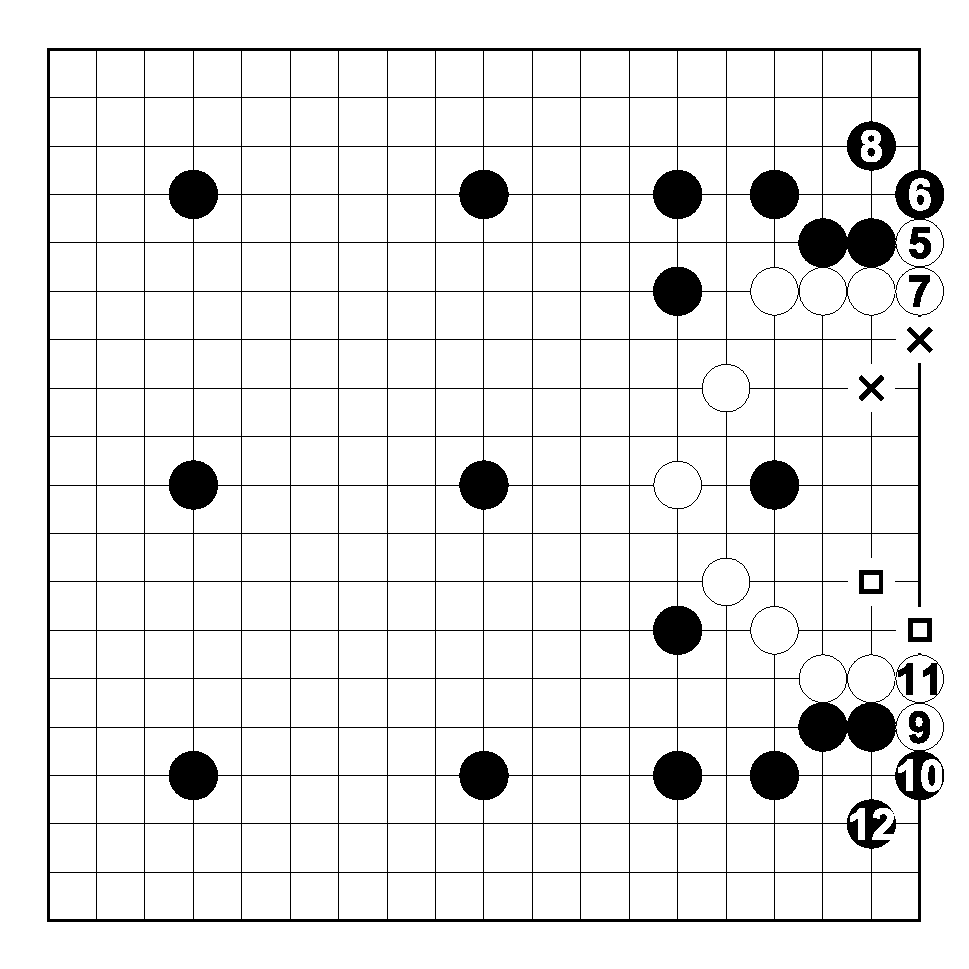
\includegraphics[width=1\textwidth]{11 - Dia 7}
        \captionsetup{justification=centering}
        \caption*{\emph{Dia.\@~7}}
    \end{subfigure}
\end{figure}

Supondo que Branco jogue como aqui, no \emph{Dia.\@~7} antes de Preto. Se Branco fizer 5, Preto precisa responder com 6. Branco conecta com 7 e Preto precisa defender com 8. Comparado a \emph{Dia.\@~6}, Branco ganhou dois pontos marcados com $\times$, e Preto perdeu dois pontos em 6 e 8. Isso é um ganho de quatro pontos para Branco\footnote{Em relação \emph{Dia. 4}, Branco possui 2 pontos a mais, e Preto, 2 a menos. No total, na comparação entre as duas sequências, temos uma diferença de $2 - (-2) = 2 + 2 = 4$.}.

Branco também termina com sente, então ele pode ainda jogar 9 e 11, forçando Preto a responder com 10 e 12. Comparado ao \emph{Dia.\@~6}, Branco ganha outros dois pontos, marcados com \(\increment\), e Preto perde dois pontos, 10 e 12. Novamente, Branco ganha quatro pontos.

Portanto, qual seja o lado que jogue seus movimentos primeiro, o ganho será de oito pontos.

\pagebreak

\begin{wrapfigure}{r}{60mm}
    \vspace{-20pt}
    \begin{center}
        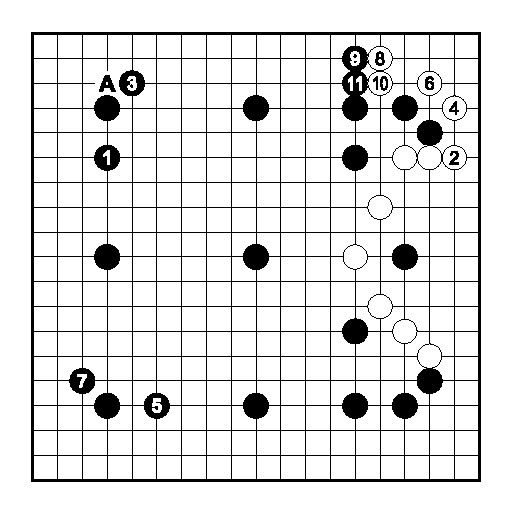
\includegraphics[width=.5\textwidth]{11 - Dia 8}
        \captionsetup{justification=centering}
        \caption*{\emph{Dia.\@~8}}
    \end{center}
    \vspace{-25pt}
\end{wrapfigure}

No entanto, a posição no \emph{Dia.\@~1} surgiu na abertura, então Preto talvez não desça para 1. Em seu lugar, ele talvez reforce sua posição no canto superior esquerdo com 1 no \emph{Dia.\@~8}. Branco talvez pense que descer para 2 é um grande movimento, já que ameaça a invasão do canto Preto, mas Preto ignoraria  tal ameaça e asseguraria o canto superior esquerdo com 3 ou \textbf{A}.

Se Branco der continuidade à ameaça de invasão ao canto superior direito preto com 4 e 6, Preto assegurará o canto inferior esquerdo com 5 e 7. A invasão branca no canto superior direito é de aproximadamente 30 pontos, mas Preto 1 a 7 delimitam um território enorme à esquerda. É difícil estimar quão grande será esse território. Branco provavelmente conseguirá invadi-lo e criar um grupo vivo, mas Preto será capaz de garantir mais de 60 pontos no processo. Sendo assim, Preto fica feliz com a troca.

O que estamos querendo enfatizar é que movimentos como Preto 1 no \emph{Dia.\@~1} e Branco 2 no \emph{Dia.\@~8} são geralmente deixados mais para o fim de jogo. Na abertura, há sempre movimentos maiores a serem feitos. É claro que Preto 1 no \emph{Dia.\@~1} é uma grande ameaça, então, do ponto de vista do Branco, ele não pode ignorá-lo. Mas, do ponto de vista do Preto, ele pode facilmente se dar ao luxo de ignorar Branco 2 no \emph{Dia.\@~8}, já que há pontos maiores em disputa do que simplesmente defender o canto\footnote{A defesa do canto é muito mais um privilégio do Preto, pois somente Preto pode se dar ao luxo de não defender.}.

O fim de jogo é um aspecto importante do jogo a se dominar. A margem de vitória ou derrota é frequentemente muito pequena, e manobras hábeis de fim de jogo podem virar a partida a seu favor.

A Kiseido já publicou dois excelentes livros sobre esse assunto. Para uma introdução detalhada ao assunto, você deveria ler o \emph{The Endgame} \cite{tomoko_bozulich_endgame}, Volume 6 da \emph{Elementary Go Series} da Kiseido. Outro livro recomendado é o \emph{Get Strong at the Endgame}~\cite{bozulich_endgame}, Volume 7 da \emph{Get Strong at Go Series} da Kiseido. Esse livro provê cálculos de fim de jogo para 101 posições básicas. Há também 120 problemas onde você deverá encontrar o tesuji de fim de jogo --- um movimento brilhante que cumpre um papel tático claro ---, que maximizará seu lucro. Ao final, há 70 problemas em tabuleiros 9\(\times\)9 e 13\(\times\)13, que lhe possiblitarão um teste de habilidade no fim de jogo.